\documentclass[sigconf,anonymous,review]{acmart}
\pdfsuppressptexinfo=-1
\hypersetup{pdfcreationdate={D:20261020000000Z},pdfmoddate={D:20261020000000Z},pdfdate={D:20261020000000Z},pdfmetadate={D:20261020000000Z}}
\usepackage{booktabs}
\usepackage{array}
\usepackage{multirow}
\usepackage{subcaption}
\usepackage{xcolor}
\newcommand{\TODO}[1]{\textcolor{red}{[TODO: #1]}}
\newcommand{\gen}[1]{\input{generated/#1}}% generated numbers only

\copyrightyear{2027}
\acmYear{2027}
\setcopyright{acmlicensed}
\acmConference[WWW '27]{Proceedings of the ACM Web Conference 2027}{May
2027}{TBD}
\acmBooktitle{Proceedings of the ACM Web Conference 2027 (WWW '27)}

\setlength{\emergencystretch}{1em}% third line-breaking pass only for paragraphs that would otherwise overflow
\makeatletter
\newcommand{\tablerows}[1]{\@@input #1.tex }
\makeatother
\begin{document}

\title{When Better Global Calibration Worsens Accepted-Set Bias:
Evidence from Web Classification under User Shift}

\begin{abstract}
Web platforms can use classifier confidence to route user-generated content:
high-confidence labels are processed automatically, while the rest are
escalated for review. Yet calibration over a whole stream need not
describe the errors among automatically processed items. We compare
scalar and conditional temperature maps in an offline routing simulation
on Amazon reviews and Yahoo Answers, with paired, exact calibration
budgets of 250 to 2{,}500 labels, and run a pre-specified external check on CivilComments.
For Amazon reviewers unseen during classifier training, at $n{=}2500$ and
a confidence threshold of $0.90$, SRTS-BCE improves ECE$_{15}$ from 3.12\%
to 2.51\% and relative whole-batch error-count error from 11.1\% to 8.6\%
over scalar TvA-TS, yet raises mean accepted-set overconfidence from
$+0.9$ to $+2.5$ percentage points. This \emph{post-hoc} mismatch occurs
in the same direction for four conditional BCE maps on two disjoint
unseen-reviewer splits that share models and calibration draws,
including at matched coverage; results on seen reviewers and Yahoo
differ. Separately, ECE rankings depend on task and label budget, and no
conditional map dominates. The absolute accepted-set bias decreases exactly when the change in
signed bias and the average of the two signed biases have opposite signs;
a positive change reduces it only where the scalar is underconfident by
more than half of that change. On CivilComments, under a protocol frozen before test
outcomes, the scalar is underconfident at high thresholds and the same
maps instead reduce the absolute accepted-set bias in 11 of 12
map--threshold settings. In simulated audits, a few hundred target labels estimate the signed
bias difference; at a 5{,}000-label cap, the evaluated joint test reaches
mean power 0.84 in the Amazon cells where the map reduces absolute bias
and 0.59 in the corresponding CivilComments cells.
Confidence-based Web routing should be audited on the accepted-set
forecast for the population it serves.
\end{abstract}

\input{metadata_candidate}

\maketitle

\section{Introduction}
\textbf{Decision setting.} Many Web services assign labels to streams of
user-generated content, such as product reviews and community questions.
Consider a confidence-based routing rule: accept a classifier's label when
its confidence exceeds a threshold, and defer the remainder for manual
verification. This is an \emph{offline decision model}, not a claim that
our benchmark platforms used such a rule. It poses a Web measurement
question: can predicted errors be trusted \emph{in the items
that automation actually handles}, including content from users absent
from training?

Two forecasts are needed: a whole-batch forecast of wrong labels in an
incoming batch, and an accepted-set forecast of the errors among
accepted labels. A low global
calibration error does not guarantee the latter: recalibration changes
confidence values and may change the accepted set itself. Moreover, a frozen classifier is
often recalibrated with few labels from its source population,
while the users it serves may change. Our experiments\footnote{Code is available at
\url{https://anonymous.4open.science/r/SRTS2026-EB80/}.} measure this gap
for review-rating and question-topic classification, with toxicity
classification as an external check (Figure~\ref{fig:reversal}); they involve no live moderation deployment
and no measured review-cost reduction.

We ask three questions:
\begin{itemize}
\item[\textbf{RQ1}] Which aggregate calibration improvements (whole-split ECE,
whole-batch error count) fail to carry over to the error forecast for the
accepted set, across label budgets, tasks and user populations?
\item[\textbf{RQ2}] How do changes in the reported scores and in the
selected items account for the discrepancy?
\item[\textbf{RQ3}] What can a small audit with labels from the served
users estimate, decide and transfer?
\end{itemize}

\textbf{Notation.} A frozen classifier maps an item $x$ to logits
$z(x)\in\mathbb R^C$, prediction $\hat y=\arg\max_c z_c$, confidence
$c=\max_c\mathrm{softmax}(z)_c$, and correctness $b=\mathbf 1[\hat y=y]$.
A calibrator is fit once on $n$ labelled pairs and keeps $\hat y$
unchanged. For a set of items $S$ we write $g(S)=\mathrm{mean}_S(c-b)$
(positive means overconfident). At threshold $t$ the auto-accept set is
$A_t=\{c\ge t\}$; $g(A_t)$ is its mean calibration bias (the gap between
predicted and actual error rates among accepted items), and the relative
whole-batch error-count error is $|g(\text{all})|/R$, with $R$ the realized
error rate. When $A_t$ and its complement are non-empty,
\begin{equation}
g(\text{all})=P(A_t)\,g(A_t)+P(A_t^c)\,g(A_t^c),
\label{eq:decomp}
\end{equation}
so a small whole-batch bias can coexist with a biased accepted set. ECE is
the 15-bin expected calibration error; TS is temperature scaling; BCE is
binary cross-entropy of $c$ against $b$. Figure~\ref{fig:reversal} shows one case: on unseen Amazon
reviewers, replacing the scalar map by SRTS-BCE lowers ECE from 3.12 to
2.51 and the whole-batch count error from 11.1\% to 8.6\%, while the
signed accepted-set bias grows from $+0.9$ to $+2.5$ points; this is one setting,
not a property of every budget or task.

\begin{figure}[t]
\centering
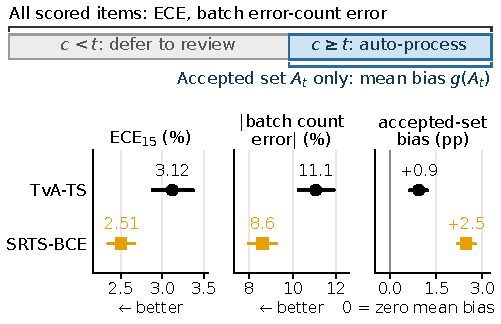
\includegraphics[width=\columnwidth]{figures/fig1_scopes.pdf}
\Description{Top: a horizontal strip of all scored items ordered by confidence c, split at the threshold t into a grey left part labelled "c < t: defer to review" and a blue right part labelled "c >= t: auto-process". A bracket over the whole strip reads "All scored items: ECE, batch error-count error"; a bracket under the blue part reads "Accepted set A_t only: mean bias g(A_t)". Bottom: three dot-and-interval panels with two rows, scalar TvA-TS (black circle) and SRTS-BCE (orange square), with numbers next to the points. ECE15 in percent: 3.12 for the scalar and 2.51 for SRTS-BCE (lower is better). Absolute relative whole-batch count error in percent: 11.1 and 8.6 (lower is better). Signed accepted-set bias in percentage points with a zero line: +0.9 and +2.5 (zero means zero mean bias), so SRTS-BCE is farther from zero.}
\caption{An illustrative endpoint reversal on unseen Amazon reviewers
($n{=}2500$, $t{=}0.90$; offline simulation, no deployed system). Top: the routing rule and its two evaluation scopes (strip widths are
schematic, not acceptance proportions); $g(A_t)$ is the mean of $c-b$
over the accepted set (positive: errors among accepted items exceed the
forecast). Bottom: replacing scalar TvA-TS with SRTS-BCE lowers
whole-split ECE$_{15}$ and the relative whole-batch error-count error but
raises the signed accepted-set bias. Means and descriptive 95\%
seed$\to$draw bootstrap intervals over 5 training runs $\times$ 20
calibration draws; each map accepts its own set (coverage 23.1\% and
26.9\%). Illustrative post-hoc comparison; Figure~\ref{fig:endpoints} reports all
four maps across three tasks.}
\label{fig:reversal}
\end{figure}
\textbf{Prior evidence and the remaining gap.} Small-sample overfitting
of flexible calibration maps is already known~\cite{balanya2024adaptive,tomani2022pts},
although SMART reports a favourable small-label regime under its own
settings~\cite{guo2026smart}. TvA and CalArena evaluate post-hoc maps on text and on large benchmarks
with random partitions~\cite{lecoz2024tva,berta2026calarena}. Distribution-shift
calibration~\cite{ovadia2019shift,desai2020calibration}, selectively
calibrated prediction~\cite{fisch2022selective}, and calibration for
downstream decisions~\cite{zhao2021decision} provide important foundations.
Deferral to congested human review has been modelled with content
moderation as the motivating case~\cite{lykouris2024defer}, and a recent
clinical study reports selective prediction degrading despite strong
aggregate metrics~\cite{lopez2026selective}. Building on these findings, we examine a narrower empirical question:
for the \emph{same prediction-preserving post-hoc maps}, do whole-batch
and threshold-accepted-set error forecasts improve consistently across
exact calibration-label budgets and previously unseen Web users?

\textbf{Contributions and evidence status.} For Amazon and Yahoo the
frozen protocol targeted the ECE comparisons of RQ1, and all other
analyses of these rows are post hoc; the CivilComments check has its own
primary family, fixed before outcomes, with one disclosed amendment
(Section~\ref{sec:civil}). (C1) \emph{Aggregate gains that miss the
accepted set (RQ1).} With exact, paired calibration draws, the Amazon
scalar--conditional ECE ordering crosses as $n$ increases, including on
1{,}334 unseen reviewers, while Yahoo favours the scalar
(Figure~\ref{fig:budget}). On two disjoint Amazon reviewer splits unseen
during backbone training, four conditional BCE maps reduce whole-batch
count error yet increase mean absolute accepted-set bias relative to a
scalar map, also at matched coverage; on seen reviewers, Yahoo and
CivilComments the direction differs (Figure~\ref{fig:endpoints}). (C2)
\emph{Scores, selection and the $D,H$ distinction (RQ2).} With $D=g_C-g_B$
the change in signed accepted-set bias and $H=(g_C+g_B)/2$, $|g|$ narrows
exactly when $DH<0$; for $D>0$, when the scalar is
underconfident by more than half of $D$ ($g_B<-D/2$). At $n{=}2500$ and $t{=}0.90$ this accounts for the contrasting seen and
unseen Amazon directions (at $t{=}0.80$ the seen-reviewer gap also widens;
Figure~\ref{fig:boundary}), and is consistent with the opposite
CivilComments result, where the scalar is
underconfident at high thresholds. On Amazon at $n{=}2500$ most of the
change is higher reported confidence on accepted items, in either accounting
order; on CivilComments a different accepted set matters
more. These are accounting identities, not causal effects. (C3) \emph{Estimation, decision and generalization (RQ3).}
Established designs estimate $D$ from a few hundred target labels if they
sample errors rather than raw correctness. Deciding whether $|g|$ shrinks
needs the sign of $H$: in the seen-reviewer cells where the
map helps, the joint $(D,H)$ test we evaluated reaches mean power 0.31,
0.58 and 0.84 under caps of 1{,}000, 2{,}500 and 5{,}000 labels
(fixed-pool inference), and 0.59 at the largest cap on CivilComments.
Across 50 reviewer partitions, full-label choices made on one half carry
over to the other with small regret (Figure~\ref{fig:closure}).
SRTS-BCE serves as a ten-coefficient risk-routed study instance; all main
maps preserve top-1 predictions. For reproducibility, the anonymized
repository provides the code, per-run results and a checker that
recomputes every quoted number.

\section{Related Work and Position}
\label{sec:related}
\textbf{Scalar and adaptive temperature maps.} Temperature scaling fits
one scalar by NLL~\cite{guo2017calibration}; TvA-TS keeps one scalar but
fits top-label BCE~\cite{lecoz2024tva}. HTS maps normalized entropy to a
temperature with two parameters and studies a family of adaptive maps at
calibration sizes down to 200~\cite{balanya2024adaptive}. PTS uses a
91-parameter network on sorted logits~\cite{tomani2022pts}; AdaTS
conditions a VAE on features~\cite{joy2023sample}; SMART regresses the
temperature on the logit margin~\cite{guo2026smart}; QaTS uses confidence
quantiles~\cite{chakraborty2026qats}. \textbf{Grouped and ensemble
calibration.} Semantic-Aware Grouping learns feature-space
partitions~\cite{yang2023semantic}, Mix-n-Match ensembles
calibrators~\cite{zhang2020mixnmatch}, Dirichlet maps with ODIR regularize
a full matrix~\cite{kull2019dirichlet}, and Meta-Cal controls
miscoverage~\cite{ma2021metacal}. \textbf{Selective prediction.}
Thresholding the maximum softmax probability is the standard selective
classification baseline~\cite{geifman2017selective}; it is evaluated by risk at a fixed coverage or by the area under the risk--coverage curve (AURC), which depend on the
ranking of confidences. Selective calibration instead requires the accepted
examples to be calibrated, measures a calibration error over confidence
levels within the accepted set, and trains a separate
selector~\cite{fisch2022selective}; selective recalibration learns a
rejector jointly with a recalibrator~\cite{zollo2024selective}. We measure a narrower quantity for a
fixed-threshold accept rule: the mean bias $g(A_t)$ of the accepted set,
which can be zero while accepted items are miscalibrated at individual
confidence levels, and which is neither an error rate nor a measure of
safety or business value. \textbf{Label-efficient evaluation.} Active
testing~\cite{kossen2021active}, including Neyman-allocated
variants~\cite{liu2026neyman}, active comparison of two
models~\cite{sawade2012active}, prediction-powered and active
inference~\cite{angelopoulos2023ppi,zrnic2024active}, and
prediction-powered active testing~\cite{ashouritaklimi2026ppat} estimate model
quality from few labels. Our audit (Section~\ref{sec:audit}) uses these designs; as in paired
model comparison, items both maps accept carry little label information
(none at matched coverage). What is specific here is the estimand, a
difference of accepted-set biases. \textbf{Position.}
Our contribution is an empirical analysis, with established calibration
maps and audit designs, of whether improvements in the calibration of
\emph{errors over a batch} extend to the \emph{mean error-rate forecast in
the selected set} across label budgets and user populations. All families above except QaTS were evaluated at matched budgets
with official code or audited ports (Appendix~\ref{app:fidelity}).

\section{Calibrators and Controls}
\label{sec:method}
\textbf{Maps compared.} The scalar maps are TS-NLL and TvA-TS (one
temperature, top-label BCE). HTS uses $T=\mathrm{softplus}(w\log\bar
H+b)$ on normalized entropy $\bar H$, fit natively by NLL or by BCE
(HTS+BCE, two coefficients). SMART maps the logit gap through a
$1{\times}16{\times}1$ network (49 coefficients), fit natively by a soft
ECE or by BCE. Margin-K3 fits one BCE temperature in each tercile of the
logit margin. SRTS-BCE and PWLinear-3 share a learned risk score,
described next.

\textbf{SRTS-BCE.} On the $n$ calibration pairs: (1)~compute six logit
statistics per sample (confidence, logit margin, probability margin,
predictive entropy, logit norm, top logit); (2)~cross-fit with five folds
an $L_2$ logistic router (sklearn, $C{=}1$, folds stratified on
correctness) for the error indicator $1-b$, with standardization moments
computed on each fold's training part, giving out-of-fold (OOF) error
scores; (3)~split the OOF scores at their $1/3$ and $2/3$ quantiles into
$K{=}3$ groups; (4)~fit one bounded BCE temperature $T_g\in[0.05,20]$ per
group, falling back to the pooled temperature for groups below 50
samples; (5)~refit router and moments on all $n$ points and route each
test item from its own logits. $K{=}1$ is exactly TvA-TS. The fitted
object has ten optimized coefficients (six router weights, an intercept,
three temperatures) plus two thresholds and twelve stored moments.
PWLinear-3 replaces step (4) by a continuous map that interpolates three
softplus-parameterized temperatures placed at the $\{1/6,1/2,5/6\}$
quantiles of the score, fit jointly by BCE; it uses the same router.

\textbf{Supporting controls.} Two nested capacity families, a
score-construction control and a local account of grouping support the
budget dependence (Appendix~\ref{app:capacity}).

\section{Experimental Setup}
\label{sec:setup}
\textbf{Web tasks.} \emph{Amazon reviews} (WILDS v2.1 official
splits~\cite{koh2021wilds}): review text $\to$ 1--5 stars, with the
reviewer as the domain variable. We train five DistilBERT
backbones~\cite{sanh2019distilbert} with the official ERM recipe and
select checkpoints on in-distribution (ID) validation accuracy only.
Out-of-distribution validation and test reviewers are disjoint from the
training reviewers and from each other (checked programmatically). The
46{,}950-review ID validation set selects the training epoch and is the
pool from which each calibration draw takes exactly $n$ labels. The ID
test split is the development split; the OOD validation set (100{,}050
reviews) is a development shift set; the OOD test set (100{,}050 reviews
from 1{,}334 reviewers with exactly 75 reviews each) is the confirmation
set. Star labels are imbalanced (60\% five stars). \emph{Yahoo Answers
topics}~\cite{zhang2015character}: 10-topic routing of question title and
content; from the official training table we carve disjoint
model-training, calibration-pool and ID-test subsets with a fixed seed;
the official test table (60{,}000 questions) is the confirmation set
(one DistilBERT architecture, three training seeds). Yahoo has no user
structure. \emph{Development
anchor}: a CIFAR-100 ViT-B/16 cell (five seeds, pool of 2{,}500) and its
95 corruption cells~\cite{hendrycks2019benchmarking}; it is never used as
confirmation.

\textbf{Exact budgets and draws.} $n\in\{250,625,1250,2500\}$ with 20
uniform draws per seed and budget (one draw when $n$ equals the pool),
exact sizes asserted; sample IDs follow from a stored seed rule and are
checked against the stored class counts and pool hash. Within a draw, all calibrators are fitted on the same $n$ labelled
examples only: standardization, routing,
thresholds, temperatures and inner model selection are refit inside the
draw.

\textbf{Endpoints.} ECE$_{15}$ (with bin-count and equal-mass
sensitivity), AdaECE~\cite{nixon2019measuring},
smECE~\cite{blasiok2023smooth}, NLL, Brier and top-label BCE; relative
whole-batch error-count error; and, at $t\in\{0.80,0.90,0.95\}$, coverage
$P(A_t)$, the actual and predicted error rate in $A_t$, $g(A_t)$, the
accepted-set relative count error $(\text{pred}-\text{actual})/\text{actual}$
and the rejected-set gap $g(A_t^c)$, which follows from
Eq.~\eqref{eq:decomp} and the whole-split fields; at matched
coverage, $g$ over each map's $\lceil qN\rceil$ most confident items, with
$q$ the scalar's coverage at $t$; risk at fixed coverage and AURC. At a fixed threshold each map accepts a different
set, so we compare how reliable each accepted set is ($|g(A_t)|$, with
its sign reported), not its error rate or coverage alone; risk at fixed
coverage compares equal-size sets and is a different estimand.

\textbf{Inference.} Six primary comparisons (SRTS-BCE versus TvA-TS and
versus SMART+BCE at $n{=}250$ and $2500$, and their budget interactions)
and all endpoints were frozen before any Web calibration result existed.
Paired per-draw deltas are summarized by a seed$\to$draw hierarchical
bootstrap; draws are never treated as independent training runs, and with
one draw per seed only seeds are resampled. With three (Yahoo) or five
(Amazon, anchor) training seeds of one architecture per task, these
intervals describe variation across these seeds and draws, and more draws
do not add training seeds; as a sensitivity toward new training runs we
also report seed-level $t$ intervals and sign agreement across seeds (Appendix~\ref{app:posthoc}). An interval that contains zero is
reported as \emph{not statistically resolved}. \emph{Access history.}
Each confirmation set was evaluated once behind a hash-verified gate; the
training scripts had also logged one backbone accuracy per seed on these
splits before the freeze, a quantity identical for every calibrator
compared there. \emph{Post-hoc analyses.} The endpoint contrasts beyond the frozen six
(on the confirmation and the development splits, and at matched coverage),
the paired seen-versus-unseen contrast, the within-family intervals and the
score-construction control were
specified in a written plan after all results had been seen; they report 95\% intervals with a Bonferroni correction over each
pre-declared family and are not independent confirmations.

\section{Results}
\label{sec:results}

\begin{table*}
\centering\footnotesize
\setlength{\tabcolsep}{3pt}
\caption{ECE$_{15}$ differences in percentage points (negative: lower ECE
for the first method), mean over seeds with 95\% hierarchical intervals. Anchor:
CIFAR-100 development cell (at $n{=}2500$ the full pool, so only seeds
vary). Amazon and Yahoo: confirmation sets, unblinded once for the frozen
primaries; later post-hoc re-evaluations are labelled as such.
$^\dagger$frozen
primary comparison; other rows are post-hoc.}
\label{tab:q1}
\begin{tabular}{lcccccc}
\toprule
& \multicolumn{2}{c}{Anchor (development)} & \multicolumn{2}{c}{Amazon,
unseen reviewers} & \multicolumn{2}{c}{Yahoo, official test}\\
\cmidrule(lr){2-3}\cmidrule(lr){4-5}\cmidrule(lr){6-7}
Comparison & $n{=}250$ & $2500$ & $n{=}250$ & $2500$ & $n{=}250$ & $2500$\\
\midrule
\tablerows{generated/q1_ece_table}
\bottomrule
\end{tabular}
\end{table*}

\subsection{RQ1: Aggregate gains that miss the accepted set}
\label{sec:rq1}



On the \emph{Amazon} confirmation set (Table~\ref{tab:q1}; budget means in Figure~\ref{fig:budget}) the
scalar has lower ECE than SRTS-BCE at $n{=}250$ and SRTS-BCE has lower ECE at $1250$ and
$2500$ (intervals exclude zero), whereas the difference at $625$ is not statistically resolved; all five seeds agree in sign at $250$, $1250$ and $2500$. Both
frozen interactions $\Delta(250)-\Delta(2500)$ exclude zero ($+0.95$
$[+0.62,\allowbreak+1.27]$ against the scalar, $-0.65$ $[-0.95,\allowbreak-0.37]$ against
SMART+BCE). At $n{=}250$ the scalar and the two-parameter HTS+BCE are
not statistically resolved ($-0.19$ $[-0.49,\allowbreak+0.16]$), and both have lower mean ECE than the 10- and 49-coefficient maps; at $n{=}2500$ the four conditional maps of Table~\ref{tab:q1} have lower mean ECE than the
scalar (the native-NLL HTS does not), and HTS+BCE has the
lowest mean ECE from $n{=}625$ on.
\begin{figure*}[t]
\centering
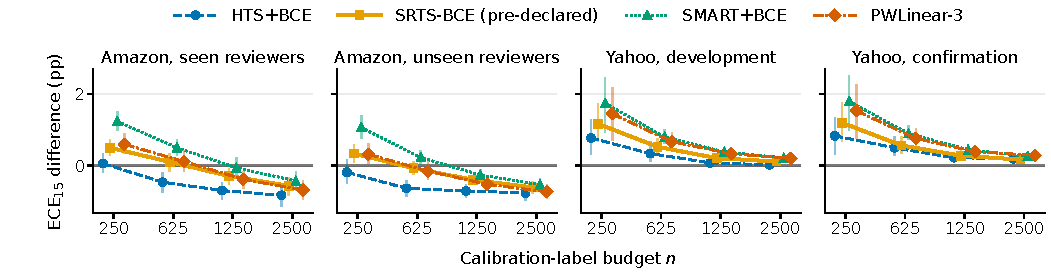
\includegraphics[width=\textwidth]{figures/fig2_budget.pdf}
\Description{Four line panels sharing a vertical axis of ECE15 difference, map minus scalar, in percentage points, with a horizontal zero line, and calibration budget 250, 625, 1250, 2500 on the horizontal axis. Panels: Amazon seen reviewers (development), Amazon unseen reviewers (confirmation), Yahoo development, Yahoo confirmation. Four lines with interval bars: HTS+BCE, SRTS-BCE, SMART+BCE, PWLinear-3. On both Amazon panels the lines start above zero at n=250 (except HTS+BCE near or below zero) and fall below zero by n=1250 or 2500, between about -0.4 and -0.9. On both Yahoo panels all lines stay above zero at every budget, decreasing from about 0.8 to 1.8 at n=250 to about 0 to 0.3 at n=2500.}
\caption{ECE rankings vary with the calibration-label budget and task: ECE$_{15}$ of each conditional map minus
the scalar TvA-TS (seen-reviewer
development split and unseen-reviewer confirmation set for Amazon;
development and confirmation sets for Yahoo). Positive: the map has higher ECE. Means over seeds
and draws with 95\% seed$\to$draw bootstrap intervals; points are offset horizontally for legibility only. SRTS-BCE $-$
scalar is the pre-declared analysis (frozen primary at $n{=}250$ and $2500$,
Table~\ref{tab:q1}; line weight marks this pre-declared comparison); the other three maps' intervals are descriptive.}
\label{fig:budget}
\end{figure*}
 The ID development split, the OOD validation reviewers and the
confirmation reviewers give the same resolution status for all ten pre-declared ECE quantities (two
comparisons at four budgets and two interactions) and the same sign for nine (the exception, SRTS-BCE versus the
scalar at $n{=}625$, is unresolved on all three), with point estimates
within $0.08$ and $0.18$ points of the ID values, so the ECE ranking transferred
from seen to unseen reviewers. On \emph{Yahoo} no conditional
map has a lower mean ECE than the scalar at any budget, and every Yahoo
comparison with the scalar in Table~\ref{tab:q1} excludes zero in the
scalar's favour; here HTS+BCE also exceeds the scalar's ECE at $n{=}250$. With three Yahoo
training seeds, seed-level $t$ intervals are wider: for the frozen SRTS-BCE versus scalar comparisons they reach zero
($[-0.04,+2.43]$ at $n{=}250$, $[-0.01,+0.33]$ at $n{=}2500$), as does
SRTS-BCE versus SMART+BCE at $n{=}250$, although all three seeds agree
in sign. SRTS-BCE has lower mean ECE than SMART+BCE at every
budget on both tasks, a gap that shrinks with $n$; under a per-task
Bonferroni correction ($1-0.05/6$) ten of the twelve confirmation
comparisons still exclude zero, the exceptions being SRTS-BCE versus
SMART+BCE at $n{=}2500$ on both tasks, and both corrected interaction intervals exclude zero.
SMART reports effectiveness with 50 validation samples in its own
configurations~\cite{guo2026smart}, a setting we did not run. In ours, both SMART variants have the two highest mean ECEs among the
main-suite maps at $n{=}250$ on all three cells, and SMART+BCE is worse
than the scalar there but better at $n{=}2500$ on the anchor and Amazon
(Table~\ref{tab:q1}). 

\begin{figure*}
\centering
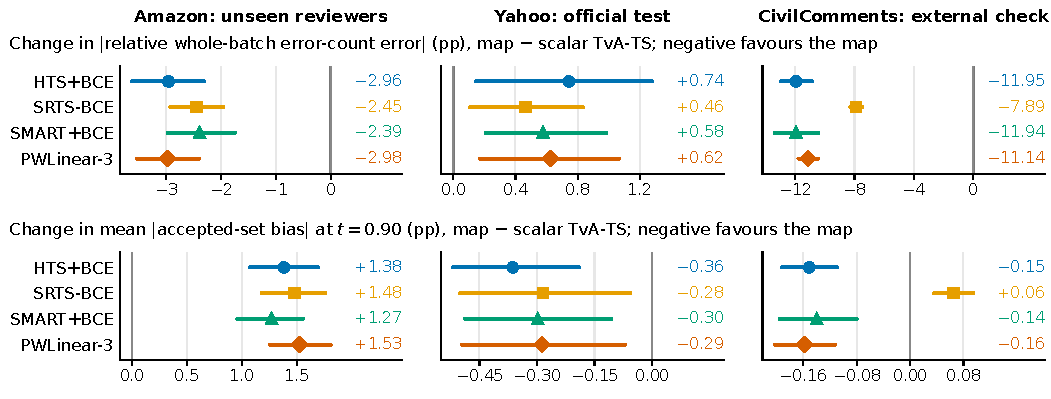
\includegraphics[width=\textwidth]{figures/fig3_tasks.pdf}
\Description{Six dot-and-interval panels in two rows and three columns (Amazon unseen reviewers, Yahoo official test, CivilComments). Each panel has four rows in the same order (HTS+BCE, SRTS-BCE, SMART+BCE, PWLinear-3), a vertical zero line and the mean printed at the right. Top row, change in the absolute relative whole-batch error-count error in percentage points, map minus scalar: Amazon -2.96, -2.45, -2.39, -2.98; Yahoo +0.74, +0.46, +0.58, +0.62; CivilComments -11.95, -7.89, -11.94, -11.14. Bottom row, change in the mean absolute accepted-set bias at threshold 0.90: Amazon +1.38, +1.48, +1.27, +1.53; Yahoo -0.36, -0.28, -0.30, -0.29; CivilComments -0.15, +0.06, -0.14, -0.16. Negative values favour the conditional map; horizontal ranges differ across panels.}
\caption{Operational effects depend on the task ($n{=}2500$, $t{=}0.90$).
Columns: Amazon unseen reviewers and Yahoo official test (confirmation
sets), CivilComments; rows: change in the relative whole-batch
error-count error and in the mean absolute accepted-set bias, each
conditional map minus scalar TvA-TS (absolute values taken per draw
before averaging); negative favours the map. Points, bars and numbers:
paired means and descriptive 95\% seed$\to$draw intervals; horizontal
ranges differ across panels. Amazon and Yahoo endpoint analyses are post
hoc (corrected inference in the text and Table~\ref{tab:q3rep}); the
CivilComments accepted-set family (bottom right) was specified before
outcomes. Full budget, threshold and matched-coverage matrix: Appendix
Figure~\ref{fig:endpoints-full}.}
\label{fig:endpoints}
\end{figure*}
\begin{table}
\centering\footnotesize
\setlength{\tabcolsep}{2.5pt}
\caption{Does the accepted-set result depend on the users? Contrasts of
the four conditional-BCE maps against the scalar. count: maps with a lower
mean whole-split count error (of 4), Bonferroni-supported in parentheses.
fixed $t$, matched: map--threshold pairs with a wider mean accepted-set
$|g|$ (of 12 = 4 maps $\times$ 3 thresholds; the others are narrower), in
parentheses Bonferroni-supported wider\,/\,narrower. Families: each
development split 32, confirmation sets 64, matched coverage 120. Post hoc;
contrasts in a cell share models, draws and test split.}
\label{tab:q3rep}
\begin{tabular}{llccc}
\toprule
Split & $n$ & count & fixed $t$ & matched\\
\midrule
\tablerows{generated/q3_replication_table}
\bottomrule
\end{tabular}
\end{table}
\textbf{Batch versus accepted-set forecasts.} Figure~\ref{fig:endpoints} shows the operating point
$n{=}2500$, $t{=}0.90$ for the three tasks; Appendix
Figure~\ref{fig:endpoints-full} gives all 64 confirmation-set contrasts of
the post-hoc plan (both budgets, three thresholds, matched coverage), and
Table~\ref{tab:q3rep} summarizes every split. On the \emph{Amazon} confirmation set every
conditional map has a lower mean whole-split count error than the scalar at
both budgets (by 1.2 to 3.0 points; 8 of 8 at 95\%, 6 of 8 after
Bonferroni), and every one has a wider mean accepted-set gap at every
threshold and budget (by 0.6 to 2.8 points; 24 of 24, all
Bonferroni-supported and all excluding zero in seed-level $t$ intervals).
At $n{=}2500$ the four maps also have the lower ECE (Table~\ref{tab:q1}),
so a better ECE and a better batch count coincide with a less reliable
accepted set; at $n{=}250$ only HTS+BCE has a lower mean ECE than the
scalar ($-0.19$, not resolved), and the other three are worse ($+0.31$ to
$+1.06$). On the OOD validation reviewers, a second disjoint set drawn from the
same source and used as a development shift split before the plan, all 24 gap means are again wider (23
Bonferroni-supported) and all 8 count means better (6 after Bonferroni).
Holding coverage equal to the scalar's within each split removes the
difference in how many items are accepted; all 24 means per unseen set stay
wider, 23 (confirmation) and 19 (OOD validation) Bonferroni-supported, so at
equal coverage the most confident items carry a larger mean bias under the
conditional maps. On reviewers seen in training (Amazon ID test) the
direction depends on budget and threshold: at $n{=}250$ all twelve
fixed-threshold means are wider (two Bonferroni-supported); at $n{=}2500$
the four at $t{=}0.80$ are wider (PWLinear-3 Bonferroni-supported) and the
eight at $t{=}0.90$ and $0.95$ narrower, three of them Bonferroni-supported
at the fixed threshold and four at matched coverage, all at $t{=}0.95$.

Through Eq.~\eqref{eq:decomp} at $t{=}0.90$, $n{=}2500$, all maps leave unseen reviewers' items overconfident; the
scalar's rejected set has a mean bias of $+3.7$ points and its accepted
set $+0.9$, while under the conditional maps the rejected-set bias is
$+2.2$ to $+2.4$ points, 0.8 to 3.8 points more items pass, and accepted
items' actual error rate exceeds the predicted one by $2.3$ to $2.5$
points (Section~\ref{sec:mechanism} accounts for the change). In
count terms, the scalar underestimates the errors among accepted items by
14\% and the conditional maps by 33--35\% (all thresholds and budgets in
Table~\ref{tab:app-endpoints}). On \emph{Yahoo} (no user-disjoint split),
the direction differs at $n{=}2500$: the conditional maps have slightly
higher batch-count errors (all four at 95\%, none after Bonferroni), but all
twelve mean gaps are narrower than the scalar's (five Bonferroni-supported,
at $t{=}0.90$ and $0.95$; likewise at matched coverage), with the scalar's
accepted set \emph{under}confident ($-0.8$ points at $t{=}0.90$) and its
whole-split count error the smallest of the five (2.4\%). At $n{=}250$ all
twelve Yahoo gap means are wider, none Bonferroni-supported, and no count
contrast is resolved. Across all 64 confirmation contrasts, 11
Bonferroni-resolved differences favour a conditional map and 24 favour the
scalar. Ranking-based endpoints move little: risk at fixed coverage
differs from the scalar's by at most $0.3$ points and AURC by at most
$0.7$ points (largest: SMART+BCE at $n{=}250$ on Amazon, resolved);
recalibration mainly changes the confidence values a threshold reads.

\textbf{A paired seen-versus-unseen contrast.} Within each map, budget,
threshold, seed and draw, $\Gamma=\Delta_{\text{unseen}}-\Delta_{\text{seen}}$
compares the change in $|g|$ on unseen and on seen reviewers for the same
fitted calibrators, with $\Delta=|g_{\text{map}}|-|g_{\text{scalar}}|$ (96
contrasts, fixed after the per-split means were known; Appendix
Table~\ref{tab:gamma}). At $n{=}2500$ and $t{=}0.90$ the maps narrow the gap
on seen reviewers by 0.19 to 0.33 points and widen it on unseen ones by 1.1
to 1.5, so $\Gamma$ is 1.45 to 1.77 points; over all 96 contrasts $\Gamma$
is positive (0.41 to 2.04 points), and the Bonferroni(96) intervals
exclude zero for 90 in two independent bootstrap streams. Resampling
evaluation reviewers as clusters makes the intervals 1.2 to 1.5 times as
wide; all eight $\Gamma$ at $n{=}2500$, $t{=}0.90$ stay above zero, but
$\Delta_{\text{seen}}$ is not statistically resolved for any map.
$\Gamma$ describes these splits, seeds and draws, not an effect of user
identity; the two unseen sets share source, models and calibration draws
(Appendix~\ref{app:posthoc}).


\subsection{RQ2: Score and Selection Accounting}
\label{sec:mechanism}
\begin{figure*}[t]
\centering
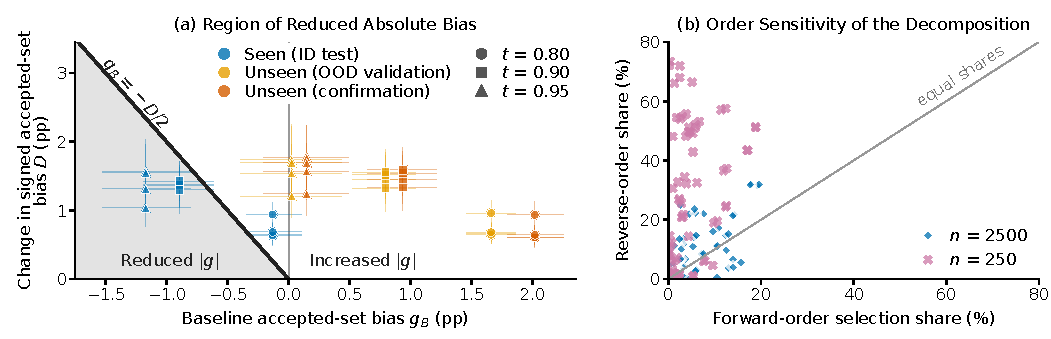
\includegraphics[width=\textwidth]{figures/fig_boundary.pdf}
\Description{Two panels. (a) Scatter plot with the scalar map's own signed accepted-set bias g_B on the horizontal axis (about -1.75 to +2.3 percentage points) and the change in signed bias D = g_map - g_scalar on the vertical axis (labelled change in signed accepted-set bias D) (0 to 3 points), for four maps, three thresholds (circles 0.80, squares 0.90, triangles 0.95) and three Amazon splits (blue seen reviewers, orange and vermilion unseen reviewers), each with horizontal and vertical interval bars. A grey wedge left of zero below the dark boundary line D = -2 g_B, labelled g_B = -D/2, marks where the absolute bias narrows. The seen-reviewer points at 0.90 and 0.95 (g_B about -0.9 and -1.2, D about 1.0 to 1.6) lie inside the wedge near its edge; the seen points at 0.80 (g_B about -0.1) and all unseen points (g_B from about 0 to +2) lie outside. (b) Scatter of the selection share in the forward order (horizontal, 0 to 80 percent) against the reverse order (vertical) with a diagonal; blue diamonds for n=2500 lie below about 20 percent forward and 32 percent reverse; pink crosses for n=250 reach up to about 73 percent in the reverse order.}
\caption{The direction of the absolute-bias change depends on the baseline bias (Amazon;
post hoc). (a) Change in signed accepted-set bias $D=g_{\text{map}}-g_{\text{scalar}}=S+P$ against the
baseline (scalar) bias $g_B$ for four maps, three thresholds and three splits
($n{=}2500$, fixed thresholds); $|g|$ narrows exactly where $DH<0$, here
(all $D>0$) the shaded wedge $g_B<-D/2$. Bars: descriptive 95\% seed$\to$draw intervals (5 seeds
$\times$ 20 draws) of each coordinate. (b) Share of the selection term in
the forward order ($P$, scalar residual) against the reverse order ($P'$,
map residual), every cell of both rules; blue diamonds $n{=}2500$, pink
crosses $n{=}250$.}
\label{fig:boundary}
\end{figure*}
In this post-hoc analysis, we decompose the change in signed accepted-set
bias into score and selection terms (Figure~\ref{fig:boundary}). For a map $C$ against the scalar $B$, with
shared correctness $b$ (every map preserves $\arg\max$, checked per draw),
\begin{equation}
\begin{aligned}
g_C(A_C)-g_B(A_B)&=S+P,\qquad S=\mathrm{mean}_{A_C}(c_C-c_B),\\
P&=\mathrm{mean}_{A_C}(c_B-b)-\mathrm{mean}_{A_B}(c_B-b),
\end{aligned}
\label{eq:account}
\end{equation}
where $S$ is the change in reported confidence on the set the map
accepts and $P$ the effect of accepting a different set, evaluated with
the scalar's residual; swapping roles ($S'$ on the scalar's set, $P'$ with
the map's residual) gives a second exact split. Neither splits
$|g_C|-|g_B|$, and the two can disagree. On Amazon at $n{=}2500$ the score
term dominates in both orders: at $t{=}0.90$, $S$ is $+1.25$ to $+1.42$ points
for the four maps on seen and on unseen reviewers, and $P$ is $+0.02$ to
$+0.08$ on seen and $+0.07$ to $+0.22$ on unseen reviewers (at most 14\%
of the change; at matched coverage at most $0.03$ points). Over all 72
cells at $n{=}2500$ $S$ ranges from $+0.55$ to $+1.54$ points with every
95\% interval above zero; the selection term is at most a fifth of the
change in the forward order, and in the reverse order the selection term
is at most a third ($+0.50$ points at $t{=}0.95$;
Figure~\ref{fig:boundary}b). At $n{=}250$ the split depends on the order
(reverse-order selection share up to 73\%), and we do not interpret it.

The direction of the change in $|g|$ follows from an exact condition.
Since $g_C^2-g_B^2=2DH$ with $D=g_C-g_B$ and $H=(g_C+g_B)/2$,
$|g_C|<|g_B|$ exactly when $DH<0$; for $D>0$, when $g_B<-D/2$: the
scalar must be underconfident by more than half the change. At
$t{=}0.90$ the change is $+1.30$ to $+1.59$ points and the scalar's
residual is $-0.89$ $[-1.19,-0.62]$ on seen and $+0.79$ / $+0.94$ on the
two unseen sets, so $|g|$ narrows on seen and widens on unseen reviewers;
at $t{=}0.80$ the seen residual ($-0.13$) is too small and $|g|$ widens
there as well (Figure~\ref{fig:boundary}a; the mean per-draw change in
$|g|$ follows the condition in all 72 cells). The seen-reviewer gains lie
close to the boundary, which makes them hard to certify
(Section~\ref{sec:audit}). This is an accounting on fixed items and fitted
maps, not a causal decomposition; it uses inspected splits and is
exploratory.

\subsection{RQ3: What a small target-label audit can estimate, decide and transfer (post hoc)}
\label{sec:audit}
\begin{figure*}[t]
\centering
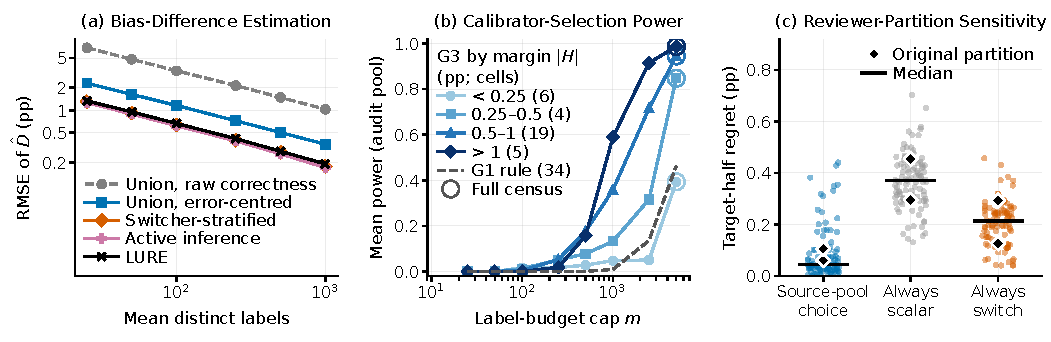
\includegraphics[width=\textwidth]{figures/fig_final_audit.pdf}
\Description{Three panels. (a) Log-log lines of the root-mean-square error of the estimated difference D against mean distinct labels (25 to 1000) on unseen reviewers for five designs: raw-correctness union sampling is highest (about 6.6 to 1 point), error-centred union sampling about 2.3 to 0.35, and switcher strata, active inference and LURE overlap at the bottom (about 1.3 to 0.18). (b) Power of the joint (D,H) test within the audit pool on seen reviewers against the label-budget cap from 25 to 5000, one line per margin stratum (below 0.25 points, 6 cells; 0.25 to 0.5, 4; 0.5 to 1, 19; above 1, 5): power stays near zero up to about 250 labels and rises to about 0.4, 0.85, 0.95 and 0.99 at the 5000 cap; rings at 5000 mark strata containing full-census cells; a dashed line for the G1 rule (corrected guardrail) over all 34 beneficial cells reaches about 0.46. (c) Strip plots over 100 reviewer partitions and directions of the mean target-half regret: the source half's full-label choice has median about 0.04 points (most below 0.2), always keeping the scalar about 0.37, always switching about 0.21; diamonds mark the original split (about 0.06 and 0.11 for the source choice).}
\caption{Estimating $D$ and detecting a beneficial change have different observed label requirements (Amazon, $n{=}2500$, fixed
thresholds; calibrators fixed at one draw per seed; post hoc). (a) RMSE
of $\hat D$ against mean distinct labels on unseen reviewers (60 cells,
400 simulated audits each); grey dashed: raw-correctness union sampling. (b) Mean
power of the joint $(D,H)$ test within the audit pool (seen reviewers;
finite-population variances) against the label-budget cap, by margin
stratum (cell counts); rings: some cells are a full census at that cap;
dashed: G1 rule (corrected guardrail), all 34 beneficial cells. (c) Reviewer-partition sensitivity: mean target-half regret in $|g|$ over 60
seen-reviewer cells for 50 reviewer partitions $\times$ 2 directions, for
the source half's full-label choice (`source-pool choice'), always keeping the
scalar and always switching, with medians (bars) and the original partition
(diamonds).
Partitions share models and population: sensitivity analyses, not
independent replications.}
\label{fig:closure}
\end{figure*}
\textbf{Setup.} For one map $C$ against the scalar $B$ at one threshold we
separate three questions: \emph{estimate} $D=g_C-g_B$ on the audited
users, \emph{decide} whether $|g_C|<|g_B|$ there, and \emph{generalize}
that decision to other users. Calibrators are fixed at one draw per seed;
reviewers are split by a hash into an audit pool and an evaluation pool.
The truth for estimation and decisions is the audit pool's full-label
value; for generalization it is the evaluation pool's. A cell whose
$||g_C|-|g_B||$ is below 0.1 points counts as equivalent (a margin fixed
in the plan). Budgets are
caps on distinct labels: designs that sample with replacement or by
Poisson sampling are charged their distinct items, and equal-label
comparisons interpolate RMSE in mean distinct labels on a log scale (plan
addenda A8--A11, Appendix~\ref{app:posthoc}).

\textbf{Estimate.} The weights
$w_i=\mathbf 1[i\in A_C]/|A_C|-\mathbf 1[i\in A_B]/|A_B|$ sum to zero,
so $D=d_{\text{conf}}+\sum_iw_ie_i$ with the label-free
$d_{\text{conf}}=\mathrm{mean}_{A_C}c_C-\mathrm{mean}_{A_B}c_B$ and errors
$e=1-b$. If each map accepts exactly the scalar's number of items
\emph{within the audited pool}, $w_i=0$ on the overlap and labelling the
switching items determines $D$ exactly: a median of 70 of about 6{,}300
accepted items on seen reviewers and 140 of 11{,}800 on unseen ones. At
fixed thresholds on unseen reviewers, switcher-stratified sampling has
RMSE $0.64$ points at 100 labels and $0.18$ at 1{,}000
(Figure~\ref{fig:closure}a). Error-centred importance sampling, active
inference with Poisson sampling~\cite{zrnic2024active} and LURE active
testing~\cite{kossen2021active} match it at equal distinct labels (RMSE
ratios 0.91 to 1.12 over both populations and all budgets), and error-centred union sampling has 1.8 to 2.5 times the RMSE of
switcher-stratified sampling; union sampling of raw correctness has 5.3 to 8.2 times the RMSE of
switcher-stratified sampling, because its sampled positive- and negative-weight terms nearly
cancel with large sampling variance: what matters is to
centre on errors and separate the signed weights, not a particular
design. Per cell, these nominal 95\% intervals have median coverage 0.94 to 0.95
from 100 labels, but their worst cells reach only 0.83 to 0.89, and error-centred union sampling has median empirical coverage of 0.63,
with a minimum of 0.13 across the evaluated cells.

\textbf{Decide.} Because $g_C^2-g_B^2=2DH$ with $H=(g_C+g_B)/2$,
$|g_C|<|g_B|$ exactly when $DH<0$; the decision needs the sign of $H$,
which weights the whole accepted sets and hence the scalar's level
$g_B$. We compare an interval rule with an Agresti--Coull level variance (G1,
the plan's corrected guardrail), a plug-in test of $H$ that estimates $D$ and ignores its
uncertainty (G2; approximate, not an oracle), and a joint $(D,H)$
intersection--union test on one stratified sample (G3), all fixed-horizon
Wald procedures. Within the audit pool (finite-population variances) on
seen reviewers, the map is better in 34 of 60 cells, worse in 20 and
within the 0.1-point margin in 6. G3 detects the better map with mean power 0.31, 0.58
and 0.84 under caps of 1{,}000, 2{,}500 and 5{,}000 labels, against 0.01,
0.14 and 0.46 for G1; false switches average at most 1\% (worst cell
4.0\%). The caps are not equal costs: at the 5{,}000 cap G3 uses 4{,}745
distinct labels on average and G1 4{,}131, and G3 labels the whole
accepted union in 19 of 60 cells, 16 of them beneficial
(Figure~\ref{fig:closure}b). Such censuses also make some of the
smallest margins resolvable, so power is not monotone in the margin. Of the 34
beneficial cells, G3 reaches 80\% power by 1{,}000 labels in 2, by
2{,}500 in 13 and by 5{,}000 in 26; 8 do not reach it at any evaluated cap. These are measured powers
of the evaluated tests, not optimal or unavoidable label requirements
(Appendix~\ref{app:posthoc} gives a conceptual identical-set example). On
unseen reviewers the map is better in 1 of 60 cells, and no corrected
procedure makes a false switch in more than 1.1\% of audits (the plan's
original guardrail: up to 45\% at 25 labels).

\textbf{Generalize.} With full labels, the better map differs between
the audit and evaluation halves in 13 of 60 seen-reviewer cells (9 when
both margins must reach 0.1 points; none on unseen reviewers). Applying the audit half's full-label choice to the other half costs 0.06 points
of $|g|$ on average, a reference choice's regret rather than a floor; the
same no-FPC G3 decisions have regret 0.10 points on the audit pool and
0.08 on the evaluation pool at the 5{,}000 cap. Across 50 salted reviewer partitions
in both directions (Figure~\ref{fig:closure}c), winner flips at a
0.1-point tolerance have median 6.5 of 60 cells (10th to 90th percentile
2 to 20); they concentrate in one training seed (41\% of its cells,
against 2 to 15\% for the others) and also arise under an item-random
split (5 flips). The audit half's full-label choice has median target
regret 0.04 points, against 0.37 for always keeping the scalar and 0.21
for always switching. Our pre-specified rule therefore does not support
a reviewer-specific failure to generalize: the flips are finite-cohort
variation in near-tie cells. The partitions share five models and one population, so they are
sensitivity summaries, not independent replications.

\subsection{External check on CivilComments (protocol frozen before outcomes)}
\label{sec:civil}
\textbf{Protocol.} Before computing any test-set result, we finalized the protocol, code and
analysis plan for binary toxicity classification on CivilComments: five DistilBERT runs with the Amazon recipe, calibration draws from a
pool that selects no checkpoint, and 95{,}502 test comments whose text is
absent from training and validation. The release has no
user or article identifiers, so this checks one fixed population, not
user transfer; one amendment before outcomes clips the HTS temperature
after 2 of 200 fits diverged (Appendix~\ref{app:civil}).

\textbf{Results.} At $n{=}2500$ every conditional map lowers ECE (by 0.47
to 1.04 points) and count error (by 7.9 to 11.9 points) and, unlike on
unseen Amazon reviewers, also lowers mean $|g|$ in 11 of 12
map--threshold cells (10 Bonferroni-resolved). In the pre-specified
family ($t{=}0.90$, Bonferroni over four maps), HTS-BCE, SMART+BCE and
PWLinear-3 reduce $|g(A_{0.90})|$ by 0.14 to 0.16 points, whereas
SRTS-BCE increases it by 0.06 $[0.03,0.10]$; each sign holds in all five runs and at matched coverage
(Figure~\ref{fig:endpoints}, right; Table~\ref{tab:civil}). The identity of RQ2 ($|g|$ narrows iff $DH<0$) accounts for the contrast with Amazon: the scalar is overconfident at
$t{=}0.80$ ($g_B{=}{+}0.38$) and underconfident at 0.90 and 0.95
($-0.26$, $-0.49$), and the sign of $DH$ from the mean $D$ and $g_B$
matches the observed change in all 12 cells, an accounting consistency
rather than an independent prediction.
Accepted items predicted toxic (simulated automatic removals) are 3.6\% of the
scalar's accepted set at $t{=}0.90$ but overconfident by 4.3 points
$[3.3,5.1]$, against $-0.44$ for accepted non-toxic items: a whole-set
forecast can hide a bias concentrated in one action.

\textbf{Audit.} Within the audit pool (accepted sets of about 42{,}000
comments, so no census), the RQ3 pattern recurs: at 100 labels switcher
strata estimate $D$ with RMSE 0.21 points (IS, active inference and LURE
0.18--0.20; raw-correctness union sampling 1.92), whereas the joint test
detects the better map in 36 beneficial cells with mean power only 0.15,
0.37 and 0.59 under caps of 1{,}000, 2{,}500 and 5{,}000 labels (false
switches at most 2.25\% per cell).

\section{Discussion and Limitations}
\label{sec:discussion}

\textbf{What the estimand covers.} We measure whether the error-rate
forecast for accepted items is accurate, not whether an item should be
accepted or review is cost-effective; the datasets contain no moderation
decisions, queues or costs, and a small mean gap does not certify
per-class, per-user or individual reliability, as the bias of simulated removals on CivilComments shows. Auditing needs labels from the served users:
at 25\% coverage each label requires screening four items; reviews
cluster by user; several maps or thresholds need a multiplicity
correction; and the $n{=}250$ calibration labels cannot serve as the
audit (only about 60 pass $t{=}0.90$, with standard error about 2.5--2.8
points at the 4--5\% accepted-set error rate of seen reviewers, and they
come from seen users). Within-pool power uses finite-population
variances, so a sample covering much of a fixed pool can resolve margins
that say nothing about other items or users; dropping that correction is
not a reviewer-level variance model. \emph{Scope.} The main finding
covers BCE-fitted temperature maps at $n{=}250$ and 2500, one
architecture per task, thresholds 0.80--0.95 and the reviewer split of
WILDS-Amazon; it does not show that conditional maps harm accepted sets
in general (CivilComments shows the opposite), that user identity causes
the difference, or which map to deploy. Each task has one backbone
family (a RoBERTa backbone on the Amazon development split reproduces the
crossing; interaction $+1.31$ $[+0.97,+1.68]$); Yahoo has three seeds and
no user structure; QaTS was not evaluated; the Amazon training epoch was
selected on the ID validation split that is also the calibration pool, a
possible confound for the sign of the scalar's residual on seen
reviewers (not re-run); and label scarcity is a study constraint, not a
measured platform quota. \emph{Inference.} The frozen Amazon and Yahoo
primaries and the CivilComments family are the only pre-specified tests;
all other analyses were planned after the results had been seen, the
matched-coverage refit reused the confirmation logits, and intervals
cover five training runs and calibration draws, not retraining with
other users, products or drift. \emph{Measurement.} ECE carries binning
caveats (we report bin and equal-mass sweeps, smECE and proper scores),
the accepted-set results hold for three thresholds, $g(A_t^c)$ is derived
through an identity, and all workflows are simulated offline.
\emph{Data and ethics.} All datasets are public research benchmarks;
there is no intervention on users; labels are re-joined from the providers by official row identifiers
rather than redistributed. A deployment would
require its own assessment of privacy, review-worker impact and
licensing.

\section{Conclusion}
A calibrator can make a batch's error forecast more accurate while
making the forecast for automatically handled items less accurate. In exploratory analyses over five training runs on two unseen-reviewer
Amazon splits, four conditional BCE maps reduce whole-batch error-count
error and, at $n{=}2500$, ECE, while increasing mean accepted-set
overconfidence relative to scalar TvA-TS, including at matched coverage;
ECE rankings depend on label budget and task. The 24 confirmation-set gap
contrasts are also supported by seed-level intervals, whereas support for
most of the 96 seen-versus-unseen contrasts relies on the seed$\to$draw
bootstrap. On Amazon at $n{=}2500$, changes in reported confidence dominate the
change in signed accepted-set bias. Absolute bias decreases
exactly when $DH<0$; for a positive bias change $D=g_C-g_B$, when
$g_B<-D/2$. On
CivilComments, where the scalar's bias differs, the same maps narrow the absolute bias in
11 of 12 settings: the direction depends on both $D$ and the scalar's bias in the
served population. In the evaluated audits, estimating such a change took far fewer labels
than deciding whether it helps: a few hundred labels estimate the signed
difference, whereas the joint test we evaluated needed caps of thousands
of labels for high power at margins of a few tenths of a point. Web
systems choosing a confidence threshold should therefore audit the error
forecast for the population and selected set they serve, separately from
global ECE and batch totals; this is a measurement recommendation, not a
validated deployment policy.

\bibliographystyle{ACM-Reference-Format}
\bibliography{references}

\appendix
\section{Baseline fidelity audits}
\label{app:fidelity}
Every baseline lists source, inputs, objective, optimizer budget,
selection rule and $\arg\max$ behaviour; all fitting labels count toward
$n$, and nothing is selected on test. \textbf{HTS}~\cite{balanya2024adaptive}: 2-parameter entropy
map $T=\mathrm{softplus}(w\log\bar H+b)$; NLL objective and a declared BCE
variant; Nelder--Mead from the matching scalar.
\textbf{PTS}~\cite{tomani2022pts}: port of the official code (pinned
commit): top-10 sorted logits $\to$ 2$\times$5 ReLU MLP $\to|T|$ (91
parameters), their MSE loss and published recipe (Adam, lr
$5{\cdot}10^{-5}$, $10^5$ steps); BCE variant reported separately.
\textbf{AdaTS}~\cite{joy2023sample}: port of the official conditional VAE
(pinned commit; their architecture, ELBO plus temperature loss and
schedule); a generic logits$\to$128$\to$1 head is not this method and is
reported as \textbf{LogitMLP-T}. \textbf{Semantic-Aware
Grouping}~\cite{yang2023semantic}: official code and defaults, combined
with TS inside $n$. \textbf{Mix-n-Match/ETS}~\cite{zhang2020mixnmatch}:
official utility path (weights reported).
\textbf{Dirichlet-ODIR}~\cite{kull2019dirichlet}: full-matrix map with
ODIR penalties tuned by inner 5-fold CV inside $n$; it changes some
predictions, which are reported, and is never excluded.
\textbf{Meta-Cal}~\cite{ma2021metacal}: miscoverage control at
$\alpha{=}0.05$ in its native semantics. \textbf{SMART}~\cite{guo2026smart}:
logit-gap $\to$ 1$\times$16$\times$1 MLP (49 parameters), native
soft-binned ECE objective and a BCE variant. All other maps preserve
$\arg\max$ (Mix-n-Match can change it only through its uniform
component).

\section{Additional tables and figures}
\label{app:tables}
\begin{figure*}[t]
\centering
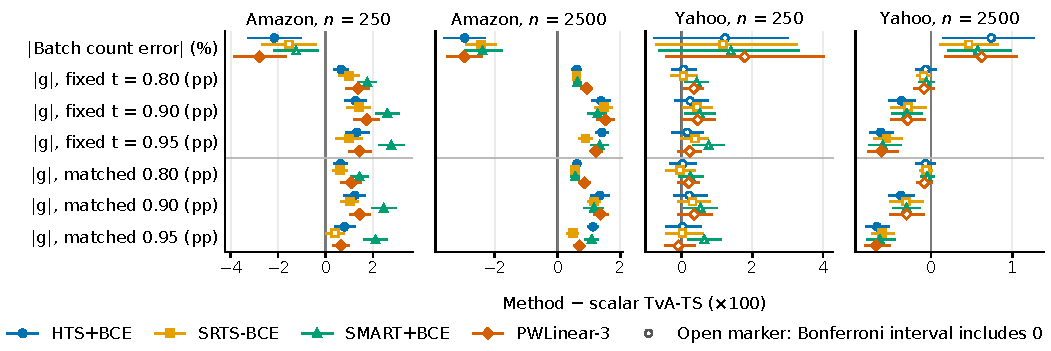
\includegraphics[width=\textwidth]{figures/endpoints_vs_scalar.pdf}
\Description{Full comparison across calibration budgets, thresholds and matched coverage. Four side-by-side dot-and-interval charts sharing one vertical list of seven endpoints: whole-split absolute relative error-count error, the absolute accepted-set gap at thresholds 0.80, 0.90 and 0.95, and the same gap at matched coverage for the three thresholds. Panels are Amazon at n=250 and n=2500 and Yahoo at n=250 and n=2500 (confirmation sets). Each panel shows, for HTS+BCE, SRTS-BCE, SMART+BCE and PWLinear-3, the difference from the scalar map times 100 with a 95 percent interval; filled markers are differences whose Bonferroni interval excludes zero. On Amazon at both budgets every method lies left of zero for the error count and right of zero for all gap rows. On Yahoo at n=250 the intervals are wide and mostly cross zero; at n=2500 the count row lies right of zero and the 0.90 and 0.95 gap rows left of zero.}
\caption{Full comparison across calibration budgets, thresholds and
matched coverage: each method
minus scalar TvA-TS ($\times100$; negative = smaller absolute error than
the scalar) on the Amazon and Yahoo confirmation sets; means over seeds with 95\% hierarchical
intervals. In this figure only, marker fill carries meaning: filled, the Bonferroni interval excludes zero, over the 64 fixed-threshold or the 120 matched-coverage contrasts of the post-hoc plan; elsewhere marker fill carries no meaning. Methods are offset within rows for legibility. PWLinear-3 is the
original construction (in-sample scores, C-IN).}
\label{fig:endpoints-full}
\end{figure*}
\begin{table}[t]
\centering\footnotesize
\setlength{\tabcolsep}{2.5pt}
\caption{Whole-split $|$count error$|$ (\%) and, per threshold, coverage
(\%) / accepted-set relative count error (\%; negative = errors among
accepted items underestimated); confirmation-set means. Where the signed gap changes sign across draws
(scalar, $n{=}250$, $t{=}0.95$) this signed mean is near zero although
the mean $|g|$ in Figure~\ref{fig:endpoints-full} is not.}
\label{tab:app-endpoints}
\begin{tabular}{lrccc}
\toprule
Method & $|$cnt$|$ & $t{=}0.80$ & $t{=}0.90$ & $t{=}0.95$\\
\midrule
\tablerows{generated/app_endpoints_table}
\bottomrule
\end{tabular}
\end{table}
Table~\ref{tab:ext} gives the faithful nearest-neighbour and extended
baselines; per-budget development-split ECE and measured calibrator cost are not
shown.
\begin{table}[t]
\centering\small
\setlength{\tabcolsep}{3pt}
\caption{Faithful nearest-neighbour/extended baselines (test
ECE$_{15}$, mean$\pm$std of per-seed means) at the anchor budgets.
Dirichlet-ODIR changes $\approx$1\% of predictions; all others preserve
$\arg\max$. AdaTS at Amazon $n{=}250$ is unstable (std 16); Mix-n-Match
(weights $(1,0,0)$) and Meta-Cal's confidence view reproduce TS-NLL.}
\label{tab:ext}
\begin{tabular}{lrrrr}
\toprule
& \multicolumn{2}{c}{Anchor (C100/ViT)} & \multicolumn{2}{c}{Amazon}\\
Method & $n{=}250$ & $2500$ & $n{=}250$ & $2500$\\
\midrule
\tablerows{generated/ext_baselines}
\bottomrule
\end{tabular}
\end{table}

\section{Capacity families and score construction}
\label{app:capacity}
\textbf{Score-construction control (post hoc).} SRTS-BCE fits its groups
on out-of-fold (OOF) router scores, whereas PWLinear-3 and the polynomial
family were fit on in-sample (IN) scores. Inside every draw we therefore
fit all four combinations of a discrete (D) or continuous (C) map with OOF
or IN scores (D-OOF = SRTS-BCE, C-IN = PWLinear-3) with the same
objective; bounds, the 50-sample floor and the optimizer stay as in the
original methods and are not matched (results: Appendix~\ref{app:posthoc}).

\textbf{Nested capacity families.} Family A splits the router score into
dyadic quantile groups $K\in\{1,2,4,8\}$ without a group-size floor;
family B maps the score through polynomials with 1--4 coefficients inside
a softplus (one coefficient is the scalar BCE map). Within each family the
signal, objective, optimizer and label access are fixed.

\textbf{A local account of grouping.} For a partition fixed independently
of the calibration sample, with per-group temperatures minimizing
empirical BCE, the expected grouped-minus-pooled population BCE is, to
leading order,
\begin{equation}
\mathbb E[\Delta]\;\approx\;-\tfrac1{2L''}\Bigl(B-\tfrac{K-1}{n}\,
\bar\sigma^2\Bigr),
\label{eq:gain}
\end{equation}
where $B$ is the between-group variance of the calibration gradient at
the pooled optimum, $\bar\sigma^2$ the within-group variance and $L''$
the curvature of the pooled objective at its optimum
(assumptions: inactive bounds, an interior pooled optimum,
curvatures and group masses bounded below, finite fourth moments, i.i.d.\
draws; proof: a second-order expansion of each group's risk with plug-in
bias $-\bar g_g/L''_g$ and variance $\sigma_g^2/(L''^2_gn_g)$, then the
expectation over multinomial group sizes). Held-out estimates of
$B/\bar\sigma^2$ are $0.0011$ to $0.0029$ on the three Yahoo seeds, below
$(K{-}1)/n=0.008$ at $n{=}250$, and $0.0045$ to $0.035$ on the five anchor
seeds; the deployed (learned, refit) router is not covered. A partition
independent of the gradient ($B{=}0$) therefore has a positive expected
cost. The statement covers only a fixed partition and the BCE objective;
it implies nothing about ECE, learned routers or shift, which are measured
empirically.

Results are in Appendix~\ref{app:posthoc} (capacity families and score construction).

\section{Post-hoc analyses: protocol, verification and additional results}
\label{app:posthoc}
\textbf{Plan.} After all results, including both confirmation sets, had
been seen, a written plan fixed the score-construction control (30
contrasts) and the 64 endpoint contrasts; dated addenda (A1--A11), each
written before its computation, added the other post-hoc analyses. \textbf{Capacity families and score
construction.} In both families and on both cells the ECE-optimal
capacity moves with $n$. The highest-capacity member minus the scalar
member is negative at $n{=}2500$ in all four family--cell pairs ($-0.44$
to $-0.63$ points) and its budget interaction is positive in all four
($+0.75$ to $+1.76$), all Bonferroni-resolved over twelve contrasts; at
$n{=}250$ it is worse than the scalar on Amazon. With the 50-sample
floor, nominal $K{=}8$ at $n{=}250$ falls back to the pooled scalar, so
the no-floor variants carry the capacity interpretation; none of this
transfers to comparisons across families. Matching the fitting scores
changes the discrete--continuous comparison little: wherever either
contrast is resolved, the matched and the original contrast agree in sign
and differ by at most $0.04$ points; cross-fitting the discrete router is
not resolved in any setting ($|\Delta|\le0.10$), and for the continuous
map OOF fitting is $0.03$ points worse, on the corruption cells only. The
map type matters by setting: the discrete map is better on the clean
anchor ($+0.06$ at $n{=}2500$, five of five seeds), the continuous map on
Amazon at $n{=}2500$ ($-0.13$, Bonferroni-resolved) and on the corruption
cells ($-0.17$; five of five seeds, but the seed-level interval includes
zero). Bounds, floor and optimizer were not matched, so the control does
not fully isolate the map type.

\textbf{Further boundaries.} With 75 reviews per OOD reviewer (below the
frozen 200-item subgroup rule), reviewer-level reliability is exploratory
(main-method differences not resolved; median per-reviewer count error
$\approx$4.9 of 75); resampling the 1{,}334 reviewers as clusters gives an
interval of $0.10$ points for SRTS-BCE minus the scalar at $n{=}2500$
(within-seed draw SD $0.26$). On the 95 corruption cells ($n{=}2500$),
SRTS-BCE minus the scalar is $-1.37$ points (five of five seeds) and minus
SMART+BCE $-0.10$ (not resolved). The one predeclared shrinkage rule
between SRTS-BCE and the scalar hedges (Amazon 3.13 vs.\ 3.09 at
$n{=}250$, 2.66 vs.\ 2.51 at $n{=}2500$); no other rule was evaluated.


\textbf{Reproduction gates.} Before any contrast was read, the new code
paths reproduced every saved SRTS-BCE row exactly and the saved
PWLinear-3 rows within $10^{-3}$ ECE points except on two Amazon draws (up
to $3.1\cdot10^{-3}$; same training objective, a flat optimum), and an
independent rebuild confirmed that every OOF score comes from a router
that did not see that item's label; the matched-coverage refit
reproduced the fixed-threshold rows to the same tolerance.
\textbf{Seed-level sensitivity.} $t$ intervals on per-seed means
(df $=$ seeds $-1$) exclude zero for 3 of the 4 frozen Amazon comparisons
at $n{=}250$ and $2500$ (not SRTS-BCE versus SMART+BCE at $n{=}2500$), 1 of
4 on Yahoo and 2 of 4 on the anchor; for 24 of 24 Amazon and 10 of 24 Yahoo
confirmation gap contrasts; for 8 of the 30 score-construction contrasts
(15 by the bootstrap); and for 9 of the 12 within-family contrasts,
including all four interactions.







\begin{table*}
\centering\footnotesize
\setlength{\tabcolsep}{3pt}
\caption{Paired seen-versus-unseen contrast at $n{=}2500$, $t{=}0.90$
(post hoc; $\times100$). $\Delta=|g_{\text{map}}|-|g_{\text{scalar}}|$ on
one split; $\Gamma=\Delta_{\text{unseen}}-\Delta_{\text{seen}}$ within each
seed and draw, same fitted calibrators. Seen: Amazon ID test; unseen: OOD validation or confirmation. Means with
95\% seed$\to$draw intervals (shared resamples); $^\ddagger$Bonferroni(96)
interval excludes zero.}
\label{tab:gamma}
\begin{tabular}{lccccc}
\toprule
& $\Delta_{\text{seen}}$ & $\Delta_{\text{unseen}}$ & $\Gamma$ &
$\Delta_{\text{unseen}}$ & $\Gamma$\\
Map & ID test & OOD validation & (OOD val.\ $-$ ID) & confirmation &
(confirm.\ $-$ ID)\\
\midrule
\tablerows{generated/gamma_rep_table}
\bottomrule
\end{tabular}
\end{table*}
\textbf{Paired seen-versus-unseen contrast.} In 94 of the 96 contrasts all
five seeds give $\Gamma>0$; the seed-level $t$ interval excludes zero in
all 96 without correction but in only one with Bonferroni correction
(df $=4$), so the family-corrected statement rests on the seed$\to$draw
bootstrap. Under reviewer-cluster resampling (plan A6; one resample of the 626,
1{,}334 and 1{,}334 reviewers shared by every model, seed and draw), the
eight $\Gamma$ at $n{=}2500$, $t{=}0.90$ have 95\% lower bounds $+0.73$ to
$+0.90$ (Bonferroni $+0.46$ to $+0.61$; 1.6 to 1.8 times as wide with
seeds and draws resampled jointly), and $\Delta_{\text{seen}}$ is not
resolved (e.g.\ HTS+BCE $-0.32$ $[-0.95,+0.52]$). In signed terms the
seen-versus-unseen difference is $-0.06$ to $+0.53$ points
(Figure~\ref{fig:boundary}). $\Gamma$ describes these
splits, seeds and draws, not an effect of user identity. It uses the matched-coverage refit, which passed its reproduction gate; a second bootstrap stream moves bounds by at most $0.033$
points. 
\textbf{Mechanism accounting and audit} (plan addenda A8--A11; post
hoc). A per-item cache of the five maps' confidences (5 seeds $\times$ 20
draws, $n\in\{250,2500\}$) reproduces the stored ECE and accepted-set gaps
exactly; Eq.~\eqref{eq:account} follows by adding and subtracting
$\mathrm{mean}_{A_C}c_B$. \emph{Accepted sets inside a pool $P$:} fixed,
$A_t=\{c\ge t\}\cap P$; exact matched coverage, each map's top $k_P$ items
of $P$, with $k_P$ the scalar's accepted count there (ties by item index;
$|A_B|=|A_C|$ asserted, so overlap weights vanish). An earlier
construction (top-$k$ on the full split, then restricted) matched counts
in only 5 of 120 audit cells and is not used.
\emph{Estimators} of $D=d_{\text{conf}}+\sum_iw_ie_i$: raw-correctness
uniform, separate-set and union samples; switcher strata (overlap,
$C\setminus B$, $B\setminus C$; allocation $\propto N_h|w_h|$;
Horvitz--Thompson, with or without an Agresti--Coull variance floor);
error-centred union and importance sampling (proposal
$\propto|w_i|\sqrt{s_i}$, 20\% defensive mixture; Hansen--Hurwitz); Poisson
sampling with AIPW as in~\cite{zrnic2024active} (inclusion
$\propto|w_i|\sqrt{s_i(1-s_i)}$; expected cost $m$); and LURE sequential
sampling without replacement as in~\cite{kossen2021active} (exactly $m$
distinct labels; approximate variance); the surrogate is $s=1-c_B$. All follow the published forms, adapted to a signed weighted total. Prediction-powered active
testing~\cite{ashouritaklimi2026ppat}, which residualizes the loss with a
prediction-powered control variate and adapts the acquisition, was not
implemented. \emph{Decisions.} With
$v_i=(\mathbf1[i\in A_C]/|A_C|+\mathbf1[i\in A_B]/|A_B|)/2$,
$H=h_{\text{conf}}-1+\sum_iv_ie_i$. G1 switches iff
$|\hat g_B+\hat D|+1.96\,\mathrm{SE}<|\hat g_B|-1.96\,\mathrm{SE}$ ($\hat
g_B$ from $m/2$ labels of $A_B$ with an Agresti--Coull variance, $\hat D$
from switcher strata); G2 is a plug-in one-sided 97.5\% test of $\hat
H=\hat g_B+\hat D/2$ that ignores $\hat D$'s uncertainty (approximate and
uncalibrated, not an oracle); G3 draws one stratified sample (allocation
$\propto N_hs_h\sqrt{w_h^2+v_h^2}$) and tests $D>0,H<0$ (or the mirror) by
intersection--union, each margin one-sided at 97.5\%. Delta-method and
power-targeted variants, the latter adapting Sawade et
al.~\cite{sawade2012active}, behave like G3 (not shown). Shared labels are
counted once. The plan's original guardrail, whose Wald level interval
has zero width when no error is observed, is reported only as a historical record.
\textbf{Proposition} (identical sets; a standard two-point reduction).
Let $A_C=A_B=A$ with $c_C=c_B+\delta$ on $A$ and $\bar\delta>0$ known.
Then $D=\bar\delta$ needs no labels, and $|g_C|<|g_B|$ iff the accuracy
$a$ on $A$ exceeds $\theta=\mathrm{mean}_Ac_B+\bar\delta/2$. If audited
labels are i.i.d.\ Bernoulli$(a)$ and nothing observed predicts them, any rule with $n$ labels whose two error probabilities at
$a=\theta\pm\epsilon$, with $0<\theta-\epsilon<\theta+\epsilon<1$, are at
most $\beta<1/2$ needs $n\ge(1-2\beta)^2r(1-r)/(2\epsilon^2)$,
$r=1-\theta-\epsilon$. \emph{Proof.} By Le Cam, the two errors sum to at
least $1-\mathrm{TV}$; Pinsker gives $\mathrm{TV}\le\sqrt{n\,\mathrm{KL}/2}$
and $\mathrm{KL}\le\chi^2=4\epsilon^2/(r(1-r))$, so
$2\beta\ge1-\sqrt{2n\epsilon^2/(r(1-r))}$; adaptive selection does not
help because every label is Bernoulli$(a)$. The assumptions exclude informative side information, the bound
decreases as $\epsilon^{-2}$ for large margins, and a census of a fixed
pool decides exactly. The construction illustrates why a choice can
remain label-dependent when $D$ is known; it does not characterize the
sample complexity of our stratified fixed-pool experiments and is not a
lower bound for the procedures above.

\section{CivilComments external check}
\label{app:civil}
\begin{table}[t]
\centering\footnotesize
\setlength{\tabcolsep}{2.2pt}
\caption{CivilComments (protocol frozen before outcomes): map minus
TvA-TS (points), means over five runs $\times$ 20 draws. $\Delta|g|$ at
$t{=}0.90$ with its seed$\to$draw interval, Bonferroni over four maps (the
pre-specified family is $n{=}2500$); matched: at the scalar's coverage;
$D=g_C-g_B$.}
\label{tab:civil}
\begin{tabular}{rlccccc}
\toprule
$n$ & Map & ECE & $|$cnt$|$\,(\%) & $|g(A_{0.90})|$ [Bonf.] & matched & $D$\\
\midrule
\tablerows{generated/civil_table}
\bottomrule
\end{tabular}
\end{table}
\textbf{Data.} With the WILDS and TensorFlow copies unreachable, we used the public
Hugging Face release (CC0; 8.0\% toxic in training). Backbones train for
one epoch on a fixed 269{,}038-comment subsample (the WILDS training
size), and the end-of-epoch model is used. Validation comments whose text appears in training are
removed; 10\% of the rest is an epoch-check slice whose accuracy is only
logged, and the other 86{,}218 form the calibration pool; draws take
exactly $n\in\{250,2500\}$ labels, 20 per run, with the Amazon seed rule.
Only the four-map family was pre-specified as a test; everything else is
descriptive. Unlike on Amazon, a different accepted set carries 0.45 to
0.87 of the change at $t{=}0.80$ (forward accounting) but at most 0.13 at
0.95. Training used 1.3 A100 GPU-hours. \textbf{Amendment.} Two of the 200 HTS-BCE fits ($n{=}250$) diverged
(coefficients near $10^{16}$), so their temperatures underflowed to zero
or tied both classes in floating point; after a diagnosis that used calibration labels and test-set logits but
no test labels, and before any test-set result was computed, the HTS
temperature was clipped to $[10^{-4},10^4]$ at prediction (the fit
already clips at $10^{-4}$). The other 198 fits are unchanged; the two are
reported as fitted.

\section{Reproducibility}
\label{app:repro}
\paragraph{Code availability.} Code is available at\\
\url{https://anonymous.4open.science/r/SRTS2026-EB80/}.
It holds the calibration, audit, analysis and training code, pinned
package versions, per-run results, number checker and layer-(A) logits;
CIFAR-100-C logits are omitted for size, and benchmark data and Web labels
must be obtained from the original providers.
\textbf{Three layers.} (A)~\emph{From logits}: Web labels and Amazon reviewer ids are re-joined to the Web logits by
official row and checked against stored SHA-256 hashes, and every calibrator and
per-run row can be recomputed on a CPU (bit-exactly except SMART, which
needs four threads, and L-BFGS-B maps, within $3\cdot10^{-3}$ ECE points). (B)~\emph{From per-run rows}: every table, figure, interval and quoted
number recomputes with fixed seeds through one command list. (C)~\emph{From data}: the training code, configurations and seeds
retrain the backbones; retraining is not bitwise reproducible. Draws use RNG $77{\cdot}10^6+10^6s+10^3n+r$, Yahoo subsets seed 20261009, and the one-time confirmation gate re-verifies the hashes of the 24 canonical scripts.

\end{document}
